\section{Introduction}
%%%%%%%%%%%%%%%%%%%%%%%%%%%%%%%%%%%%%%%%%%%%%%%%%%%%%%%%%%%%%%%%%%%%%%%%
%%%%%%%%%%%%%%%%%% MOTIVATION & BACKGROUND SECTION %%%%%%%%%%%%%%%%%%
%%%%%%%%%%%%%%%%%%%%%%%%%%%%%%%%%%%%%%%%%%%%%%%%%%%%%%%%%%%%%%%%%%%%%%%%

\begin{figure}[t]
    \centering
    \resizebox{0.99\columnwidth}{!}{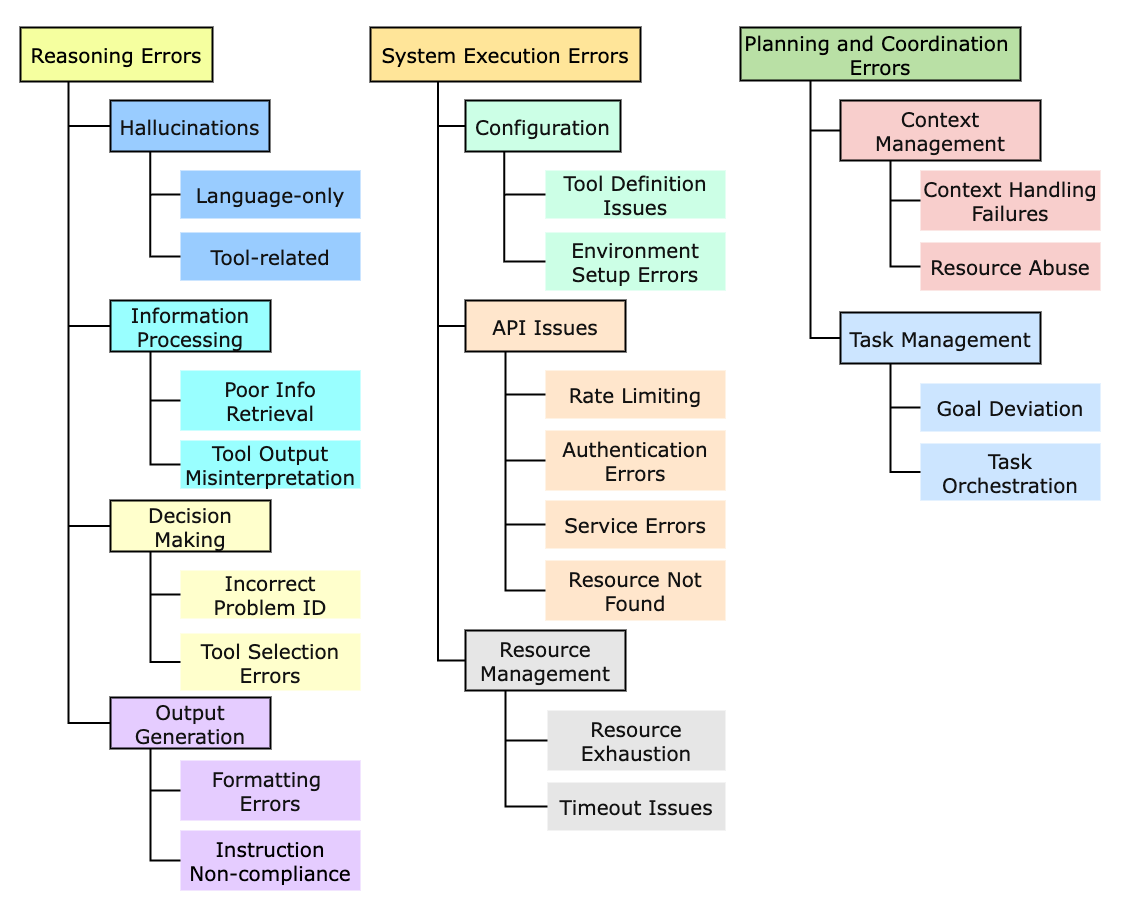
\includegraphics{figures/diagrams/trail_taxonomy.png}}
    \vspace{-0.4cm}
    \caption{Illustration of the TRAIL taxonomy of errors}
    \label{fig:trail_taxonomy}
    \vspace{-0.4em}
\end{figure}

The rapid advancement of large language models (LLMs) has catalyzed the development of agentic systems capable of automating difficult, multi-step tasks across various domains such as software engineering and multi-hop IR \cite{ma2023laser, OpenAI2024DeepResearch, nguyen2024dynasaur, wang2025browsing}. Unlike traditional generative models, agents can interact with diverse tools and dynamically navigate environments, often with minimal human supervision~\cite{wang2024survey}. This escalation of system complexity demands more challenging and multifaceted evaluation processes~\cite{nasim2025governance} and has led to the adoption of LLMs as evaluators for such agentic systems \cite{zheng2023judging, chen2024mllmjudge, kim-etal-2024-prometheus, zhu2025judgelm, deshpande2024glider}. 

However, as multi-agent systems scale and become integral to real-world workflows, evaluating and debugging their performance remains a significant challenge. Agentic non-determinism~\cite{laban2025llms,patronus2025statistical_risk} and multi-step task solving~\cite{mialon2023gaia,yao2024tau} demand greater observability than the simple end-to-end evaluations offered by existing benchmarks~\cite{kapoor2024ai, zhuge2024agent, moshkovich2025beyond, cemri2025multi}. Such complex environments require granular taxonomies and well-annotated traces that can serve as references for debugging and root-cause analysis of agent behaviors~\cite{cemri2025multi}.
When creating taxonomies and benchmarks to test and improve agents, we must ensure these are grounded in real-world applications and are not centered around dummy data~\cite{bowman2021will, liu2024ecbd}. Previous agent trace analysis frameworks have primarily focused on parsed traces containing unstructured text~\cite{cemri2025multi}, which do not adequately represent common agent framework outputs that generate structured traces logged in standardized formats like \texttt{opentelemetry}~\cite{opentelemetry}. Additionally, as observed by ~\citet{guo2023gpt4graph, sui2024tablellm}, handling structured data remains challenging for LLMs, an observation corroborated by previous research on automated software engineering trace analysis ~\cite{roy2024exploring, ma2024llmparser}. These limitations highlight the need for new approaches specifically designed for structured agentic traces.
To address these challenges and facilitate the analysis and evaluation of agentic executions, we propose a formal error taxonomy, shown in~\autoref{fig:annotation_categories}, that promotes granular failure diagnosis. We also present a carefully curated, turn-level annotated trace dataset called \textsc{TRAIL} (Trace Reasoning and Agentic Issue Localization), which demonstrates the validity and practical utility of our proposed taxonomy.

%%%%%%%%%%%%%%%%%%%%%%%%%%%%%%%%%%%%%%%%%%%%%%%%%%%%%%%%%%%%%%%%%%%%%%%%
%%%%%%%%%%%%%%%%%% SWE Bench %%%%%%%%%%%%%%%%%%
%%%%%%%%%%%%%%%%%%%%%%%%%%%%%%%%%%%%%%%%%%%%%%%%%%%%%%%%%%%%%%%%%%%%%%%%

In our work, we utilize and build on SWE-Bench \cite{jimenez2024swebench, aleithan2024swebenchplus} and GAIA \cite{mialon2023gaia} while addressing three major shortcomings inherent to previous automatic agent evaluation paradigms. Firstly, we aim to replace end to end analysis of agents with a benchmark containing step-level analysis of traced agentic workflows. Secondly, we address the need for grounding in real scenarios by producing \texttt{opentelemetry}-based structured traces that span beyond present model context length limits. Finally, as compared to benchmarks focused only on agentic reasoning and coordination~\cite{cemri2025multi, kokel2025acp}, \textsc{TRAIL} focuses on validity through addition of finer, more aligned system execution failures and planning error categories such as \textit{API errors} and \textit{Task Orchestration Errors} to our taxonomy. Such categories are not only relevant to model developers but also to users and engineers optimizing single and multi-agent AI applications. 
%%%%%%%%%%%%%%%%%%%%%%%%%%%%%%%%%%%%%%%%%%%%%%%%%%%%%%%%%%%%%%%%%%%%%%%%
%%%%%%%%%%%%%%%%%% 3. CONTRIBUTION SUMMARY SECTION %%%%%%%%%%%%%%%%%%
%%%%%%%%%%%%%%%%%%%%%%%%%%%%%%%%%%%%%%%%%%%%%%%%%%%%%%%%%%%%%%%%%%%%%%%%
The contributions of our work are as follows:
\begin{itemize}[itemsep=1mm, parsep=0.5pt]
    \item We introduce a formal taxonomy (\autoref{fig:trail_taxonomy}) that defines, fine-grained agentic error categories spanning across three key areas: reasoning, planning, and execution.
    \item Based on this taxonomy, we present \textsc{TRAIL}, an ecologically grounded execution trace benchmark comprising 148 meticulously curated traces (totaling 1987 open telemetry spans, of which 575 exhibit at least one error) drawn from the GAIA \cite{mialon2023gaia} and SWE-Bench \cite{jimenez2024swebench} datasets and covering a wide range of tasks.
    \item We show that \textsc{TRAIL} is a non-trivially difficult benchmark for LLMs on many fronts
    \begin{enumerate}
        \item Current SOTA LLM families such as \textsc{o3}, \textsc{claude-3.7-sonnet} and \textsc{gemini-2.5-pro} perform modestly at best on \textsc{TRAIL}, both in terms of predicting error categories and their location. With \textsc{gemini-2.5-pro} the best performing model, achieving only 11\% combined joint accuracy on both splits.
        \item Solving \textsc{TRAIL} requires a significant fraction of the maximum input length of LLMs (or exceeds it), as well as requires generating  significant fraction of their maximum output (See \autoref{tab:token_length_analysis}, Figure \ref{fig:length_distributions})
        \item Models benchmarked on \textsc{TRAIL} benefit from both the presence and greater extent of reasoning chains (\S \ref{subsubsec:reason_vs_nonreason}, \S \ref{subsubsec:reasoning_effort}), highlighting the need for improvement in exploration capabilities of LLMs.
    \end{enumerate} 
    \item \textsc{TRAIL} is fully open-source (MIT License), will be accompanied by a HuggingFace leaderboard, and serves as a foundation for future research on evaluating agentic workflows.
\end{itemize} 


% - Agent systems we use - multi and single agents
% - Trace - Openinference format
% - Taxonomy 